\documentclass[tikz,border=10pt]{standalone}
\usepackage{amsmath}
\usepackage{tikz}
\usetikzlibrary{arrows.meta, positioning, calc, shapes.geometric}

\begin{document}
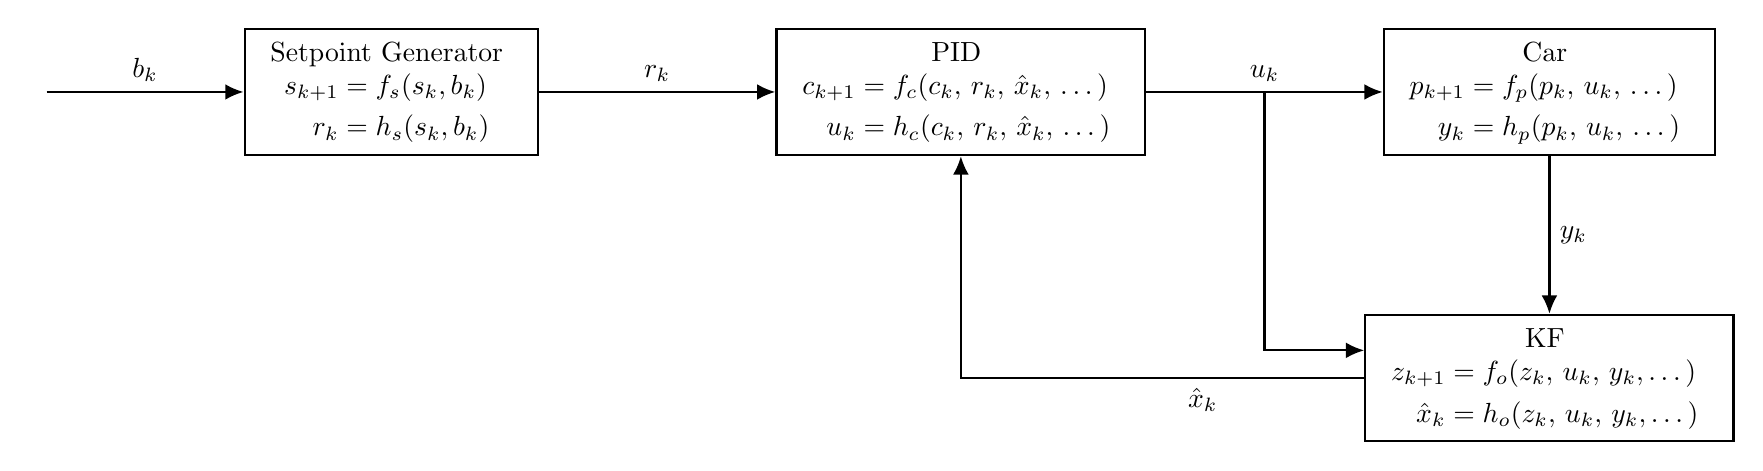
\begin{tikzpicture}[
  block/.style = {draw, thick, minimum height=3em, minimum width=6em, align=center},
  arrow/.style = {thick, -{Latex[width=2mm]}},
  node distance=2.5cm and 2.5cm
]

  % Signal Generator
  \node[block] (siggen) {
    \begin{tabular}{c}
       Setpoint Generator \\
      $\begin{aligned}
      s_{k+1} &= f_s(s_k,b_k) \\
      r_{k} &= h_s(s_k,b_k)
       \end{aligned}$
    \end{tabular}
  };

  % Controller (now directly takes r and xhat)
  \node[block, right=3.0cm of siggen] (controller) {
    \begin{tabular}{c}
            PID\\
      $\begin{aligned}
      c_{k+1} &= f_c(c_k,\,r_k,\,\hat{x}_k,\,\dots) \\
      u_k &= h_c(c_k,\,r_k,\,\hat{x}_k,\,\dots)
       \end{aligned}$      
    \end{tabular}
  };

  % Plant
  \node[block, right=3.0cm of controller] (system) {
    \begin{tabular}{c}
      Car\\      
      $\begin{aligned}
      p_{k+1} &= f_p(p_k,\,u_k,\,\dots) \\
      y_k &= h_p(p_k,\,u_k,\,\dots)
       \end{aligned}$                  
    \end{tabular}
  };

  % Observer
  \node[block, below=2cm of system] (observer) {
    \begin{tabular}{c}
      KF\\      
    $\begin{aligned}
      z_{k+1} &= f_o(z_k,\,u_k,\,y_k,\dots) \\
      \hat{x}_{k} &= h_o(z_k,\,u_k,\,y_k,\dots)
       \end{aligned}$            
    \end{tabular}
  };

  % bk -> signal
  \node[left=2.5cm of siggen] (button) {};
  \draw[arrow] (button.east) -- node[above] {$b_k$} (siggen.west);

  % r -> controller
  \draw[arrow] (siggen.east) -- node[above] {$r_k$} (controller.west);

  % controller -> plant
  \draw[arrow] (controller.east) -- node[above] {$u_k$} (system.west);

  % u branch to observer
  \coordinate (usplit) at ($(controller.east)!0.5!(system.west)$);
  \coordinate[above=1em of observer.west] (observer_uin);
  \draw[arrow] (usplit) |- (observer_uin) node[pos=0.25, right] {};

  % y_p -> observer
  \draw[arrow] (system.south) -- node[right] {$y_k$} (observer.north);

  % observer -> controller (state estimate)
  \coordinate (controller_yoin) at ($(controller.south)!0.5!(controller.south -| observer.north)$);
  \draw[arrow] (observer.west) -| node[pos=0.2, below] {$\hat{x}_k$} (controller.south);

\end{tikzpicture}
\end{document}
